\documentclass[aspectratio=169,10pt,t]{beamer}
\usepackage[utf8]{inputenc}
\usepackage[T1]{fontenc}
\usepackage{amsmath,amssymb}
\usepackage{booktabs,array,tabularx,multirow}
\usepackage[table]{xcolor}
\usepackage{pgfplots}
\pgfplotsset{compat=1.17}
\usepackage{tikz}
\usetikzlibrary{arrows.meta,positioning,calc,shapes.geometric,fit,decorations.pathreplacing}

\definecolor{azul}{HTML}{1F4E79}
\definecolor{azulc}{HTML}{E8F0F8}
\definecolor{azulm}{HTML}{5B8DB8}
\definecolor{verde}{HTML}{2E7D32}
\definecolor{verdec}{HTML}{E9F5EA}
\definecolor{naranja}{HTML}{C75B12}
\definecolor{naranjac}{HTML}{FDF1E6}
\definecolor{rojo}{HTML}{B3261E}
\definecolor{gris}{HTML}{666666}
\definecolor{grisc}{HTML}{F3F3F3}

\setbeamercolor{normal text}{fg=black!85}
\setbeamercolor{structure}{fg=azul}
\setbeamercolor{alerted text}{fg=naranja}
\setbeamercolor{block title}{bg=azul,fg=white}
\setbeamercolor{block body}{bg=azulc,fg=black!85}
\setbeamercolor{block title alerted}{bg=naranja,fg=white}
\setbeamercolor{block body alerted}{bg=naranjac,fg=black!85}
\setbeamercolor{block title example}{bg=verde,fg=white}
\setbeamercolor{block body example}{bg=verdec,fg=black!85}
\setbeamerfont{block title}{size=\small,series=\bfseries}
\setbeamertemplate{navigation symbols}{}
\setbeamertemplate{itemize item}{\color{azul}\small$\blacktriangleright$}
\setbeamertemplate{itemize subitem}{\color{azulm}\scriptsize$\blacktriangleright$}
\setbeamertemplate{enumerate item}{\color{azul}\insertenumlabel.}
\setbeamertemplate{blocks}[rounded][shadow=false]

\setbeamertemplate{frametitle}{%
  \vskip-0.1cm
  \begin{tikzpicture}[remember picture,overlay]
    \fill[azul] (current page.north west) rectangle ([yshift=-1.15cm]current page.north east);
    \fill[naranja] ([yshift=-1.15cm]current page.north west) rectangle ([yshift=-1.21cm]current page.north east);
    \node[anchor=west,text=white,font=\Large\bfseries] at ([xshift=0.7cm,yshift=-0.58cm]current page.north west) {\insertframetitle};
  \end{tikzpicture}\vskip0.55cm}
\setbeamertemplate{footline}{%
  \hfill{\color{gris}\scriptsize Autoencoder recurrente de ciclos de marcha \quad \insertframenumber/\inserttotalframenumber}\hspace{0.6cm}\vskip0.25cm}
\setbeamersize{text margin left=0.8cm,text margin right=0.8cm}

\newcommand{\gr}{$^\circ$}
\newcommand{\mae}{\ensuremath{\mathrm{MAE}}}
\newcommand{\bpm}[2]{$\mathbf{#1}\boldsymbol{\pm}\mathbf{#2}$}
\newcommand{\men}{\textcolor{naranja}{\textbf{Menor}}}
\newcommand{\ok}{\textcolor{verde}{\textbf{Sí}}}
\newcommand{\no}{\textcolor{rojo}{\textbf{No}}}
\newcommand{\neu}{\textcolor{naranja}{\textbf{Neutro}}}

% grafico de barras horizontales manual
\newcommand{\barchart}[3]{%
\begin{tikzpicture}[x=#2,y=-#3]
 \foreach \lab/\val/\cls [count=\i from 0] in {#1}{
  \ifnum\cls=1 \def\col{azul}\else\def\col{gris!55}\fi
  \node[anchor=east,font=\scriptsize] at (-0.12,\i) {\lab};
  \fill[\col] (0,\i-0.32) rectangle (\val,\i+0.32);
  \node[anchor=west,font=\scriptsize] at (\val+0.05,\i) {\val};
 }
\end{tikzpicture}}

\title{Autoencoder recurrente sobre ciclos de marcha}
\subtitle{Diagnóstico, mejoras validadas y lo que no funcionó}
\author{Práctica Investigativa III}
\institute{Seguimiento del avance}
\date{Noviembre de 2026}

\begin{document}

%--------------------------------------------------------------------
\begin{frame}[plain]
\begin{tikzpicture}[remember picture,overlay]
 \fill[azul] (current page.south west) rectangle (current page.north east);
 \fill[naranja] ([yshift=-0.14cm]current page.south west) rectangle ([yshift=0.0cm]current page.south east);
 \node[anchor=west,text=white,align=left,text width=0.85\paperwidth] at ([xshift=1.2cm,yshift=0.6cm]current page.west) {\fontsize{24}{28}\selectfont\bfseries Autoencoder recurrente\\ sobre ciclos de marcha\\[8pt]\large\mdseries Diagnóstico, mejoras validadas y lo que no funcionó};
 \node[anchor=west,text=white!85,align=left,font=\small] at ([xshift=1.2cm,yshift=-2.2cm]current page.west) {Práctica Investigativa III\\ Seguimiento del avance -- noviembre de 2026};
\end{tikzpicture}
\end{frame}

%--------------------------------------------------------------------
\begin{frame}{Resumen en una diapositiva}
\begin{columns}[T]
\begin{column}{0.5\textwidth}
\begin{block}{Qué se encontró}
\begin{itemize}\small\setlength{\itemsep}{2pt}
\item Se trabajó con una misma red recurrente (GRU) en dos variantes: \textbf{A}, entrenada con ciclos limpios (reconstruir), y \textbf{B}, entrenada con ciclos dañados (corregir). Ambas tenían el mayor error entre los modelos que aprenden de los datos en la comparación inicial.
\item Dos defectos fueron identificados: \alert{olvido} del código en el decodificador y \alert{ciclos que no cierran}.
\item Dos cambios pequeños los corrigieron. La mejora fue validada con 5 semillas y prueba t pareada.
\item La mayoría de las ideas adicionales no aportó mejoras; eso acota dónde está el límite (datos).
\end{itemize}
\end{block}
\end{column}
\begin{column}{0.48\textwidth}
\centering\footnotesize\setlength{\tabcolsep}{3pt}
\begin{tabular}{@{}lccc@{}}
\toprule
 & \textbf{Inicial} & \textbf{1 modelo} & \textbf{Ensamble}\\
\midrule
A: \mae{} (\gr) & 5.17 & 4.11 & \textbf{3.91}\\
A: salto (\gr) & 4.94 & 0.87 & \textbf{0.55}\\
B: \mae{} (\gr) & 5.35 & 4.83 & \textbf{4.74}\\
B: salto (\gr) & 3.45 & 0.57 & \textbf{0.36}\\
B: corrección & 0.280 & 0.337 & \textbf{0.349}\\
\bottomrule
\end{tabular}

\vspace{4pt}
{\scriptsize 1 modelo: promedio de 5 semillas. Ensamble: promedio de las predicciones de 5 modelos (un solo ensamble). Ambos modelos se evalúan con las mismas métricas. Negrilla: mejor cifra de cada fila.}
\end{column}
\end{columns}
\end{frame}

%--------------------------------------------------------------------
\begin{frame}{Contexto: qué es un ciclo y qué se pretende}
\begin{columns}[T]
\begin{column}{0.5\textwidth}
\begin{itemize}\setlength{\itemsep}{4pt}
\item Un \alert{ciclo de marcha} es una zancada completa, remuestreada a 101 puntos (0--100\% del ciclo).
\item Seis ángulos sagitales: cadera, rodilla y tobillo, izquierda y derecha. Cada ciclo es una matriz $G\in\mathbb{R}^{101\times 6}$.
\item Datos: 461 ciclos válidos de 64 personas, estimados por video a 30 fps.
\end{itemize}
\vspace{4pt}
\begin{block}{Dos usos del modelo}
\textbf{Fidelidad}: reconstruir un ciclo con el menor error posible.\\
\textbf{Corrección}: dado un ciclo atípico, devolver una versión típica.
\end{block}
\end{column}
\begin{column}{0.48\textwidth}
\centering
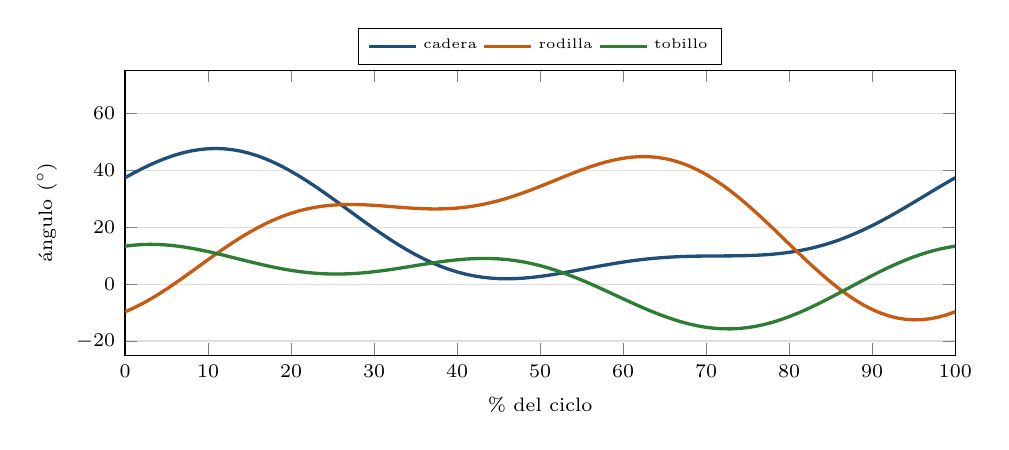
\begin{tikzpicture}
\begin{axis}[width=\textwidth,height=5.2cm,xlabel={\% del ciclo},ylabel={ángulo (\gr)},
 xmin=0,xmax=100,ymin=-25,ymax=75,legend style={font=\tiny,at={(0.5,1.02)},anchor=south,legend columns=3},
 tick label style={font=\scriptsize},label style={font=\scriptsize},ymajorgrids,grid style={gray!25}]
\addplot[azul,very thick,domain=0:100,samples=101]{20+20*sin(deg(2*pi*x/100)+60)+8*sin(deg(4*pi*x/100))};
\addlegendentry{cadera}
\addplot[naranja,very thick,domain=0:100,samples=101]{20+22*sin(deg(2*pi*x/100)-90)+12*sin(deg(4*pi*x/100)-40)};
\addlegendentry{rodilla}
\addplot[verde,very thick,domain=0:100,samples=101]{2+10*sin(deg(2*pi*x/100)+20)+8*sin(deg(4*pi*x/100)+100)};
\addlegendentry{tobillo}
\end{axis}
\end{tikzpicture}

{\scriptsize Ilustración esquemática de un ciclo (no son datos reales).}
\end{column}
\end{columns}
\end{frame}

%--------------------------------------------------------------------
\begin{frame}{El autoencoder: comprimir y reconstruir}
\centering
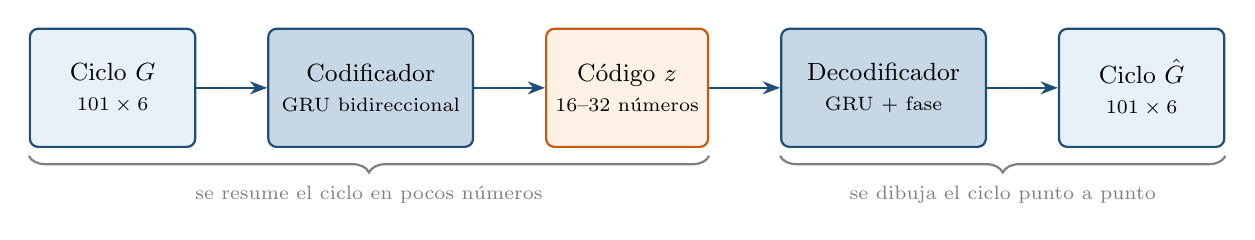
\begin{tikzpicture}[node distance=0.9cm,
 caja/.style={draw=azul,fill=azulc,rounded corners=3pt,minimum height=1.5cm,align=center,font=\small,thick},
 flecha/.style={-{Stealth[length=2.2mm]},thick,azul}]
\node[caja,minimum width=2.1cm] (in) {Ciclo $G$\\ \scriptsize $101\times6$};
\node[caja,right=of in,minimum width=2.6cm,fill=azulm!35] (enc) {Codificador\\ \scriptsize GRU bidireccional};
\node[draw=naranja,fill=naranjac,thick,rounded corners=3pt,right=of enc,minimum width=1.5cm,minimum height=1.5cm,align=center,font=\small] (z) {Código $z$\\ \scriptsize 16--32 números};
\node[caja,right=of z,minimum width=2.6cm,fill=azulm!35] (dec) {Decodificador\\ \scriptsize GRU + fase};
\node[caja,right=of dec,minimum width=2.1cm] (out) {Ciclo $\hat G$\\ \scriptsize $101\times6$};
\draw[flecha] (in)--(enc); \draw[flecha] (enc)--(z); \draw[flecha] (z)--(dec); \draw[flecha] (dec)--(out);
\draw[decorate,decoration={brace,amplitude=6pt,mirror},thick,gray] ([yshift=-0.1cm]in.south west) -- node[below=7pt,font=\scriptsize,gray]{se resume el ciclo en pocos números}([yshift=-0.1cm]z.south east);
\draw[decorate,decoration={brace,amplitude=6pt,mirror},thick,gray] ([yshift=-0.1cm]dec.south west) -- node[below=7pt,font=\scriptsize,gray]{se dibuja el ciclo punto a punto}([yshift=-0.1cm]out.south east);
\end{tikzpicture}

\vspace{10pt}
\begin{columns}[T]
\begin{column}{0.48\textwidth}
\begin{block}{Analogía}
Describir una canción en una frase y pedir a otra persona que la tararee a partir de esa frase. Si la frase es buena, la melodía se recupera.
\end{block}
\end{column}
\begin{column}{0.48\textwidth}
\begin{block}{Pérdida original}
Error cuadrático medio entre $G$ y $\hat G$ (ángulos estandarizados). Nada en esa pérdida exige que $\hat G$ sea \emph{periódico}.
\end{block}
\end{column}
\end{columns}
\end{frame}

%--------------------------------------------------------------------
\begin{frame}{De dónde vienen los modelos: A y B}
\begin{columns}[T]
\begin{column}{0.56\textwidth}
\footnotesize
\renewcommand{\arraystretch}{1.15}
\begin{tabularx}{\textwidth}{@{}>{\ttfamily\raggedright\arraybackslash}p{3.7cm}>{\raggedright\arraybackslash}X@{}}
\toprule
\textnormal{\textbf{Nombre en el cuaderno}} & \textbf{Nombre aquí}\\
\midrule
control\_mean & media de controles\\
pca & PCA\\
autoencoder\_1d & autoencoder convolucional\\
denoising\_autoencoder\_1d & autoencoder convolucional denoising\\
\rowcolor{naranjac}\textbf{rnn\_autoencoder} & \textbf{modelo A}\\
\rowcolor{naranjac}\textbf{denoising\_rnn\_autoencoder} & \textbf{modelo B}\\
gp\_periodic\_residual & proceso gaussiano periódico\\
\bottomrule
\end{tabularx}
\end{column}
\begin{column}{0.42\textwidth}
\begin{block}{Cuaderno de origen}\scriptsize
\texttt{10\_cycle\_manifold\_models.ipynb}\\
Ruta: \texttt{01-experimentation/notebooks/}\\
Datos: generados por \texttt{09\_cycle\_manifold\_data\_preparation.ipynb}\\
Resultados: \texttt{01-experimentation/outputs/cycle\_manifold\_models/}
\end{block}
\begin{exampleblock}{A y B: misma red, distinto entrenamiento}\scriptsize
\textbf{A}: recibe ciclos limpios y debe devolverlos.\\
\textbf{B}: recibe ciclos dañados (amplitud, desplazamiento, ruido, corrimiento de fase) y debe devolver el ciclo limpio.
\end{exampleblock}
\end{column}
\end{columns}
\end{frame}

%--------------------------------------------------------------------
\begin{frame}{Qué mide cada métrica (las mismas para todos los modelos)}
\footnotesize
\renewcommand{\arraystretch}{1.15}
\begin{tabularx}{\textwidth}{@{}>{\raggedright\arraybackslash}p{2.6cm}>{\raggedright\arraybackslash}p{3.6cm}>{\raggedright\arraybackslash}p{2.6cm}>{\raggedright\arraybackslash}X@{}}
\toprule
\textbf{Evaluación} & \textbf{Datos} & \textbf{Métrica} & \textbf{Lectura}\\
\midrule
\textbf{I. Fidelidad} & 47 ciclos limpios de control no vistos & \mae{} (\gr) & error medio punto a punto; menor es mejor\\
 & & Salto de cierre (\gr) & $|$salida(0\%) $-$ salida(100\%)$|$; menor es mejor\\
\textbf{II. Corrección} & los mismos ciclos, dañados artificialmente & Ganancia de corrección & $1-\frac{\mae(\text{salida},\text{limpio})}{\mae(\text{dañado},\text{limpio})}$; mayor es mejor\\
\textbf{III. Casos externos} & 130 ciclos del grupo de casos & Ganancia de tipicidad & $1-d_{\text{salida}}/d_{\text{entrada}}$, $d$ = distancia al control más cercano; mayor es mejor\\
 & & Intervención (\gr) & cuánto cambia la salida respecto a la entrada (no hay ``mejor'')\\
\bottomrule
\end{tabularx}

\vspace{2pt}
\begin{block}{A y B no tienen métricas distintas}\small
Todas las métricas se aplican a todos los modelos. Cambia \emph{en cuáles destaca cada uno}: A fue entrenado para copiar (se compara sobre todo en I) y B para corregir (se compara sobre todo en II). Si una tabla muestra solo algunas métricas, son las que el cambio probado podía mover.
\end{block}
\end{frame}

%--------------------------------------------------------------------
\begin{frame}{Punto de partida: comparación inicial de modelos}
\centering\footnotesize\setlength{\tabcolsep}{5pt}
\begin{tabular}{lccccc}
\toprule
 & \textbf{\mae{} (\gr)} & \textbf{Salto (\gr)} & \textbf{Corrección} & \textbf{Tipicidad} & \textbf{Intervención (\gr)}\\
\midrule
Media de controles & 8.77 & \textbf{0.60} & $-0.121$ & 0.132 & 10.83\\
PCA & \textbf{2.78} & 3.41 & 0.207 & 0.127 & 3.86\\
Autoencoder convolucional & 3.30 & 3.11 & 0.252 & 0.182 & 4.83\\
Autoencoder convolucional denoising & 4.07 & 1.88 & \textbf{0.412} & 0.376 & 5.98\\
Proceso gaussiano periódico & 3.30 & \textbf{0.60} & 0.215 & 0.192 & 3.86\\
\rowcolor{naranjac}\textbf{Modelo A} & 5.17 & 4.94 & 0.152 & 0.349 & 8.12\\
\rowcolor{naranjac}\textbf{Modelo B} & 5.35 & 3.45 & 0.280 & \textbf{0.385} & 7.89\\
\bottomrule
\end{tabular}

\vspace{6pt}
\begin{columns}[T]
\begin{column}{0.48\textwidth}
\begin{block}{Qué se observa}\scriptsize
Entre los modelos que aprenden de los datos, A y B tienen el mayor error y los mayores saltos. B tiene la mayor ganancia de tipicidad (0.385); la mayor ganancia de corrección es la del autoencoder convolucional denoising (0.412).
\end{block}
\end{column}
\begin{column}{0.48\textwidth}
\begin{block}{Nota}\scriptsize
Cifras del cuaderno original, conjunto de control no visto (fidelidad, corrección) y casos externos (tipicidad, intervención). A y B tienen las cinco columnas. Negrilla: mejor valor de la columna (el salto de 0.60 de la media de controles es trivial: promedia ciclos).
\end{block}
\end{column}
\end{columns}
\end{frame}

\begin{frame}{Diagnóstico: dos causas probables del bajo desempeño}
\begin{columns}[T]
\begin{column}{0.49\textwidth}
\begin{alertblock}{1. Olvido}
El código $z$ solo entra como estado inicial. Tras 101 pasos, la memoria se diluye.

\smallskip
\emph{Analogía}: dictar una dirección una única vez y esperar que se recuerde cien pasos después.

\smallskip
\textbf{Remedio}: entregar $z$ en cada paso.
\end{alertblock}
\end{column}
\begin{column}{0.49\textwidth}
\begin{alertblock}{2. El ciclo no cierra}
La pérdida solo mide error punto a punto. Si el último punto queda lejos del primero, no hay castigo específico.

\smallskip
\emph{Analogía}: una curva que no se une consigo misma deja una ``costura'' visible al encadenar zancadas.

\smallskip
\textbf{Remedio}: penalizar $|\hat G(0)-\hat G(100)|$.
\end{alertblock}
\end{column}
\end{columns}
\vspace{2pt}
\centering
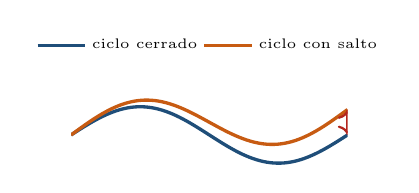
\begin{tikzpicture}
\begin{axis}[width=0.42\textwidth,height=2.8cm,hide axis,xmin=0,xmax=1,ymin=-1.4,ymax=2,
 legend style={font=\tiny,draw=none,at={(0.5,1.15)},anchor=south,legend columns=2}]
\addplot[azul,very thick,domain=0:1,samples=80]{sin(deg(2*pi*x))};
\addlegendentry{ciclo cerrado}
\addplot[naranja,very thick,domain=0:1,samples=80]{sin(deg(2*pi*x))+0.9*x};
\addlegendentry{ciclo con salto}
\draw[<->,thick,rojo] (axis cs:1,0) -- node[right,font=\scriptsize,rojo]{salto} (axis cs:1,0.9);
\end{axis}
\end{tikzpicture}
\hspace{0.3cm}{\scriptsize Ilustración esquemática.}
\end{frame}

%--------------------------------------------------------------------
\begin{frame}{Protocolo de evaluación}
\begin{columns}[T]
\begin{column}{0.5\textwidth}
\begin{block}{Datos y entrenamiento}
\begin{itemize}\setlength{\itemsep}{2pt}\small
\item Partición \alert{por sujeto} (sin fuga entre ciclos de una misma persona).
\item Entrenamiento: 240 ciclos / 28 sujetos. Validación: 44 / 6. Prueba de control: 47 / 7. Casos externos: 130 / 23.
\item Estandarización con estadísticas del entrenamiento.
\item Optimizador adaptativo (tasa $10^{-3}$), lote 64, hasta 100 épocas, parada temprana (paciencia 12), 48 unidades ocultas.
\end{itemize}
\end{block}
\end{column}
\begin{column}{0.48\textwidth}
\begin{block}{Tres evaluaciones}
\begin{enumerate}\setlength{\itemsep}{2pt}\small
\item[I.] Reconstrucción de ciclos limpios (\mae{}, salto).
\item[II.] Corrección de ciclos \emph{dañados} artificialmente (ganancia de corrección).
\item[III.] Casos externos (tipicidad e intervención).
\end{enumerate}
\end{block}
\begin{exampleblock}{Regla de validación}
Explorar con una semilla; afirmar solo con \textbf{cinco semillas} (42, 1, 7, 123, 2024) y prueba t pareada.
\end{exampleblock}
\end{column}
\end{columns}
\end{frame}

%--------------------------------------------------------------------
\begin{frame}{Por qué cinco semillas}
\begin{columns}[T]
\begin{column}{0.5\textwidth}
\begin{itemize}\setlength{\itemsep}{4pt}
\item Con 240 ciclos de entrenamiento, una misma configuración cambia de resultado según el azar inicial.
\item El RNN original fluctuó $\pm0.23$\gr{} en \mae{} y $\pm0.55$\gr{} en salto.
\item Una mejora de décimas observada con una sola semilla \alert{no es evidencia}.
\item Cada variante fue comparada \emph{semilla a semilla}; el valor $p$ resume si la ventaja se repite.
\end{itemize}
\end{column}
\begin{column}{0.48\textwidth}
\begin{block}{Ejemplo: mismo modelo, cinco semillas}
\centering\small
\begin{tabular}{rcc}
\toprule
Semilla & \mae{} (\gr) & Salto (\gr)\\
\midrule
42 & 4.182 & 1.140\\
1 & 4.208 & 1.494\\
7 & 4.234 & 1.198\\
123 & 4.178 & 1.358\\
2024 & 4.176 & 1.433\\
\bottomrule
\end{tabular}

\scriptsize Runa repetida + cierre, latente 16. El salto varía de 1.14 a 1.49 sin cambiar nada más.
\end{block}
\end{column}
\end{columns}
\end{frame}

%--------------------------------------------------------------------
\begin{frame}{Mapa de experimentos}
\begin{columns}[T]
\begin{column}{0.47\textwidth}
\begin{exampleblock}{Funcionan (5 semillas; 7: un ensamble)}
\small
\begin{tabular}{@{}rlc@{}}
1 & Código en cada paso & \ok\\
2 & Pérdida de cierre & \ok\\
3 & Ambos juntos & \ok\\
5 & Extensión a denoising & \ok\\
6 & Latente 32, $w=0.1$ (A) & \ok\\
7 & Ensamble de 5 semillas & \ok\\
\end{tabular}
\end{exampleblock}
\end{column}
\begin{column}{0.52\textwidth}
\begin{alertblock}{No confirmados}
\small
\begin{tabular}{@{}rlc@{}}
4 & Suavidad (1.ª y 2.ª diferencia) & \no\\
8 & Decodificador bidireccional & \no\\
9 & Atención en el codificador & \no\\
10 & Velocidad / asimetría como entrada & \no\\
11 & Consistencia del latente & \neu\\
12 & Intensidad y currículo de corrupción & \neu\\
13 & Peso de cierre $w=0.07$ (denoising) & \men\\
14 & Latentes 32/48/64 (denoising) & \neu\\
15 & Ensamble mixto A + B & \no\\
16 & Otras lecturas de $t$ y $t-1$ & \neu\\
17 & Modelo fundacional congelado & \no\\
18 & Codificador lineal (control) & \textcolor{naranja}{\textbf{Mixto}}\\
\end{tabular}
\end{alertblock}
\end{column}
\end{columns}
\vspace{2pt}
{\scriptsize Neutro: diferencia dentro del ruido o sin significancia. Menor: mejora pequeña (salto $0.57\to0.47$, $p=0.022$). El 16 mejora la forma de la curva, no el error. Mixto: mejor \mae{} que el GRU, peor cierre.}
\end{frame}

%--------------------------------------------------------------------
\begin{frame}{Mejora 1: el código en cada paso del decodificador}
\centering
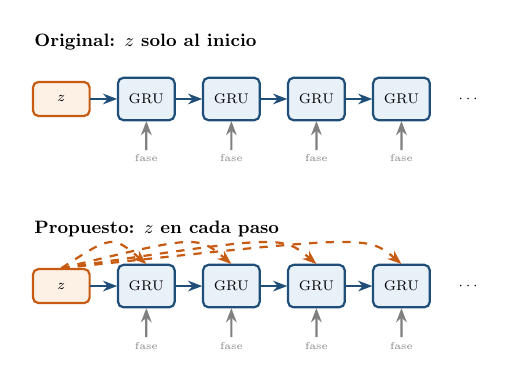
\begin{tikzpicture}[scale=0.72,every node/.append style={transform shape},
 cel/.style={draw=azul,fill=azulc,rounded corners=2pt,minimum width=1.0cm,minimum height=0.75cm,font=\scriptsize,thick},
 zb/.style={draw=naranja,fill=naranjac,rounded corners=2pt,minimum width=1.0cm,minimum height=0.6cm,font=\scriptsize,thick},
 ar/.style={-{Stealth[length=1.8mm]},thick,azul}]
% original
\node[font=\small\bfseries,anchor=west] at (-0.2,2.1) {Original: $z$ solo al inicio};
\node[zb] (z0) at (0.4,1.1) {$z$};
\foreach \i in {1,...,4}{\node[cel] (a\i) at (0.4+1.5*\i,1.1) {GRU};}
\node[font=\scriptsize] at (7.6,1.1) {$\cdots$};
\draw[ar] (z0)--(a1); \foreach \i/\j in {1/2,2/3,3/4}{\draw[ar] (a\i)--(a\j);}
\foreach \i in {1,...,4}{\draw[ar,gray] (0.4+1.5*\i,0.2)--(a\i); \node[font=\tiny,gray] at (0.4+1.5*\i,0.05) {fase};}
% mejorado
\begin{scope}[yshift=-3.3cm]
\node[font=\small\bfseries,anchor=west] at (-0.2,2.1) {Propuesto: $z$ en cada paso};
\node[zb] (zz) at (0.4,1.1) {$z$};
\foreach \i in {1,...,4}{\node[cel] (b\i) at (0.4+1.5*\i,1.1) {GRU};}
\node[font=\scriptsize] at (7.6,1.1) {$\cdots$};
\draw[ar] (zz)--(b1); \foreach \i/\j in {1/2,2/3,3/4}{\draw[ar] (b\i)--(b\j);}
\foreach \i in {1,...,4}{\draw[ar,gray] (0.4+1.5*\i,0.2)--(b\i); \node[font=\tiny,gray] at (0.4+1.5*\i,0.05) {fase};
 \draw[ar,naranja,dashed] (zz.north) .. controls (0.4+1.5*\i-0.6,2.0) .. (b\i.north);}
\end{scope}
\end{tikzpicture}

\vspace{4pt}
\begin{columns}[T]
\begin{column}{0.48\textwidth}
\begin{block}{Intuición}\small
Es la diferencia entre dictar la receta una sola vez y tenerla a la vista durante toda la cocción.
\end{block}
\end{column}
\begin{column}{0.48\textwidth}
\begin{exampleblock}{Resultado (una semilla)}\small
\mae{}: \textbf{4.84\gr\ $\to$ 4.22\gr}. El salto baja poco (4.75\gr\ $\to$ 3.9\gr): mejora la fidelidad, no el cierre.
\end{exampleblock}
\end{column}
\end{columns}
\end{frame}

%--------------------------------------------------------------------
\begin{frame}{Mejora 2: penalizar que el ciclo no cierre}
\begin{columns}[T]
\begin{column}{0.44\textwidth}
\begin{block}{Pérdida}
\[
\mathcal{L}=\underbrace{\operatorname{mean}(\hat G-G)^2}_{\text{fidelidad}}+w\,\underbrace{\operatorname{mean}|\hat G(0)-\hat G(100)|}_{\text{cierre}}
\]
\end{block}
\begin{itemize}\setlength{\itemsep}{3pt}\small
\item El peso $w$ regula la exigencia del cierre.
\item Existe un \alert{compromiso}: $w$ grande fuerza el cierre pero resta libertad a la curva.
\item Se selecciona un valor pequeño (0.05--0.1): el salto cae de 4.75\gr\ a 2.3--1.0\gr\ y el error cambia poco (una semilla).
\end{itemize}
\end{column}
\begin{column}{0.54\textwidth}
\centering
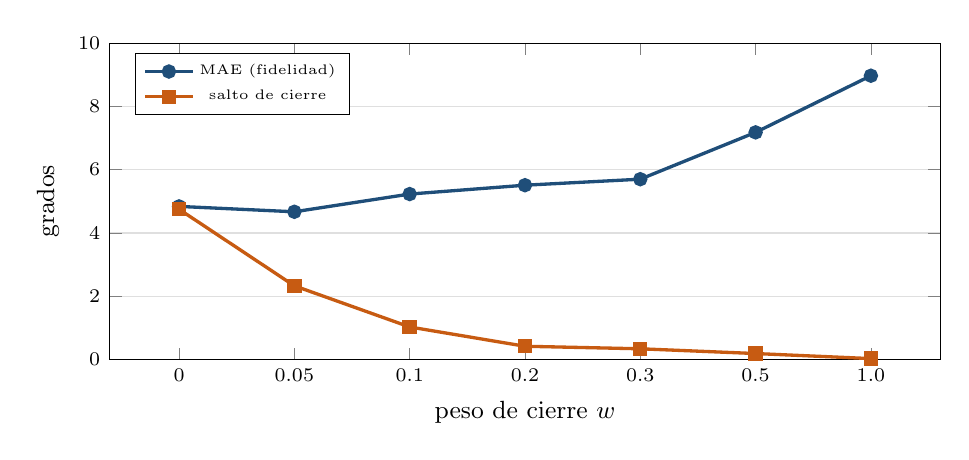
\begin{tikzpicture}
\begin{axis}[width=\textwidth,height=5.6cm,xlabel={peso de cierre $w$},ylabel={grados},
 symbolic x coords={0,0.05,0.1,0.2,0.3,0.5,1.0},xtick=data,ymin=0,ymax=10,
 legend style={font=\tiny,at={(0.03,0.97)},anchor=north west},
 tick label style={font=\scriptsize},label style={font=\small},ymajorgrids,grid style={gray!25}]
\addplot[azul,mark=*,very thick] coordinates {(0,4.84)(0.05,4.67)(0.1,5.23)(0.2,5.51)(0.3,5.70)(0.5,7.18)(1.0,8.97)};
\addlegendentry{\mae{} (fidelidad)}
\addplot[naranja,mark=square*,very thick] coordinates {(0,4.75)(0.05,2.33)(0.1,1.03)(0.2,0.42)(0.3,0.34)(0.5,0.19)(1.0,0.03)};
\addlegendentry{salto de cierre}
\end{axis}
\end{tikzpicture}

{\scriptsize Pérdida de cierre aplicada sola, una semilla.}
\end{column}
\end{columns}
\end{frame}

%--------------------------------------------------------------------
\begin{frame}{Mejoras 1 + 2 juntas: validación con cinco semillas}
\begin{columns}[T]
\begin{column}{0.46\textwidth}
\small
\begin{tabular}{lcc}
\toprule
 & \textbf{\mae{} (\gr)} & \textbf{Salto (\gr)}\\
\midrule
RNN original (reproducido) & $4.99\pm0.23$ & $5.07\pm0.55$\\
\rowcolor{verdec}Código por paso + cierre & \bpm{4.20}{0.03} & \bpm{1.33}{0.15}\\
\bottomrule
\end{tabular}

\vspace{6pt}
\begin{exampleblock}{Lectura}
\begin{itemize}\setlength{\itemsep}{2pt}\small
\item Gana en las 5 semillas, en ambas métricas.
\item La dispersión cae de $\pm0.23$ a $\pm0.03$: el modelo es además \alert{mucho más estable}.
\item Las dos mejoras son complementarias: una reduce error, la otra cierra el ciclo.
\end{itemize}
\end{exampleblock}
\end{column}
\begin{column}{0.52\textwidth}
\centering
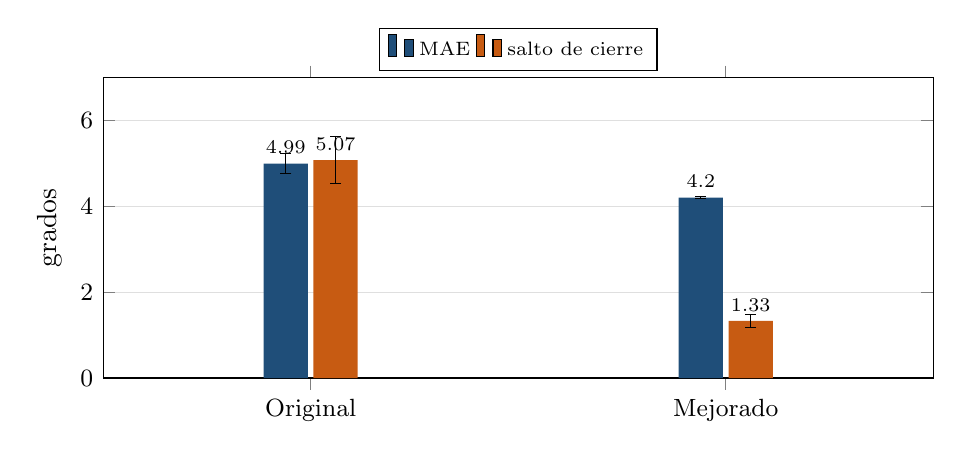
\begin{tikzpicture}
\begin{axis}[ybar,width=\textwidth,height=5.4cm,bar width=16pt,symbolic x coords={Original,Mejorado},xtick=data,
 ymin=0,ymax=7,ylabel={grados},enlarge x limits=0.5,
 legend style={font=\scriptsize,at={(0.5,1.02)},anchor=south,legend columns=2},
 tick label style={font=\small},nodes near coords,nodes near coords style={font=\scriptsize},
 every node near coord/.append style={/pgf/number format/fixed,/pgf/number format/precision=2},ymajorgrids,grid style={gray!25}]
\addplot[fill=azul,draw=none,error bars/.cd,y dir=both,y explicit] coordinates {(Original,4.99) +- (0,0.23) (Mejorado,4.20) +- (0,0.03)};
\addplot[fill=naranja,draw=none,error bars/.cd,y dir=both,y explicit] coordinates {(Original,5.07) +- (0,0.55) (Mejorado,1.33) +- (0,0.15)};
\legend{\mae{},salto de cierre}
\end{axis}
\end{tikzpicture}

{\scriptsize Media $\pm$ desviación estándar, 5 semillas.}
\end{column}
\end{columns}
\end{frame}

%--------------------------------------------------------------------
\begin{frame}{Sugerencia: penalizar la diferencia entre $t$ y $t-1$}
\begin{columns}[T]
\begin{column}{0.5\textwidth}
\begin{block}{Lo probado}
Penalización sobre diferencias consecutivas de la salida (suavidad) y sobre la segunda diferencia (aceleración), sola y combinada con el cierre.
\end{block}
\small
\begin{tabular}{lccc}
\toprule
Peso de suavidad & 0 & 0.2 & 3.0\\
\midrule
\mae{} (\gr) & 4.219 & \textbf{4.215} & 4.451\\
Salto (\gr) & 3.912 & \textbf{3.907} & 5.862\\
\bottomrule
\end{tabular}

\vspace{4pt}
{\scriptsize Una semilla. Aceleración y combinación con cierre: mismo patrón (\mae{} 4.18 en todos los casos).}
\end{column}
\begin{column}{0.47\textwidth}
\begin{alertblock}{Por qué no aporta}
Una GRU ya produce salidas suaves: su estado cambia gradualmente. Se pedía algo que ya se cumplía.
\end{alertblock}
\begin{exampleblock}{Qué sí captura la idea}
El problema no estaba \emph{dentro} del ciclo sino en la \alert{costura}: el vecino anterior ($t-1$) del punto 0 es el punto 100. Esa diferencia, que cruza el borde, es precisamente la pérdida de cierre.
\end{exampleblock}
{\scriptsize Otras lecturas: siguientes diapositivas.}
\end{column}
\end{columns}
\end{frame}

%--------------------------------------------------------------------
\begin{frame}{Otras lecturas de $t$ y $t-1$}
\scriptsize
\renewcommand{\arraystretch}{1.15}
\begin{tabularx}{\textwidth}{@{}>{\raggedright\arraybackslash}p{2.7cm}>{\raggedright\arraybackslash}X>{\raggedright\arraybackslash}p{5.1cm}@{}}
\toprule
\textbf{Lectura} & \textbf{Intuición} & \textbf{Resultado exploratorio (1 semilla)}\\
\midrule
Suavidad circular & Penalizar $|\hat G_t-\hat G_{t-1}|$ contando también el paso del punto 100 al 0 & Cierra solo en parte: salto 3.1\gr\ frente a 3.9\gr\ sin nada y 1.1\gr\ con la pérdida de cierre\\
Curvatura circular & Penalizar la segunda diferencia: evitar ``esquinas'', también en la costura & Baja pendiente en la costura y rugosidad; el error no cambia\\
Igualar incrementos & Exigir que el cambio de $t-1$ a $t$ se parezca al \emph{real}, no solo el valor & Mejora levemente el error en incrementos; el salto de cierre sube\\
Pendiente en la costura & Exigir que la pendiente final iguale la inicial (continuidad de la derivada) & Pendiente 1.38 $\to$ 0.13, con pequeño costo en error\\
Kernel periódico & Puntos cercanos en fase circular deben tener valores cercanos (como en el proceso gaussiano) & Con peso fuerte el error sube a 4.98\gr; con peso suave no aporta\\
Peso por fase & Más peso al error cerca de los extremos del ciclo & Error 4.11\gr, pero el salto de cierre sube a 3.3\gr\\
\bottomrule
\end{tabularx}

\vspace{6pt}
\normalsize
\begin{block}{Nuevas métricas de forma (grados; menor es mejor)}\scriptsize
\textbf{Pendiente en la costura}: diferencia entre pendiente final e inicial (``quiebre'' visible al encadenar zancadas). \textbf{Error en incrementos}: si los cambios paso a paso se parecen a los reales. \textbf{Rugosidad}: promedio de la segunda diferencia.
\end{block}
\end{frame}

%--------------------------------------------------------------------
\begin{frame}{Otras lecturas: validación con cinco semillas}
\footnotesize\setlength{\tabcolsep}{3pt}
\centering
\begin{tabular}{lccccc}
\toprule
 & \mae{} & Salto & Pend. costura & Err. increm. & Rugosidad\\
\midrule
Referencia, $w=0.05$ & \bpm{4.20}{0.03} & $1.33\pm0.15$ & $1.15\pm0.19$ & $0.578\pm0.007$ & $0.118\pm0.003$\\
Referencia, $w=0.1$ & $4.24\pm0.03$ & \bpm{0.83}{0.07} & $1.15\pm0.16$ & $0.581\pm0.008$ & $0.118\pm0.004$\\
\rowcolor{verdec}Incrementos, $w=0.1$ & $4.21\pm0.03$ & $0.99\pm0.12$ & $0.70\pm0.09$ & $0.557\pm0.005$ & $0.110\pm0.002$\\
\rowcolor{verdec}Incrementos + curvatura & $4.21\pm0.03$ & $0.95\pm0.10$ & $0.58\pm0.07$ & \bpm{0.553}{0.003} & $0.104\pm0.002$\\
Incrementos + pendiente & $4.24\pm0.06$ & $0.96\pm0.06$ & \bpm{0.19}{0.02} & \bpm{0.553}{0.006} & $0.106\pm0.001$\\
Curvatura (peso 3), $w=0.05$ & $4.25\pm0.03$ & $0.96\pm0.09$ & $0.52\pm0.04$ & $0.567\pm0.007$ & \bpm{0.094}{0.002}\\
\midrule
Ciclos reales & -- & 6.0 & 0.81 & -- & 0.226\\
\bottomrule
\end{tabular}

\vspace{6pt}
\begin{columns}[T]
\begin{column}{0.52\textwidth}
\begin{exampleblock}{Lectura}\scriptsize
Con el mismo $w=0.1$, igualar incrementos reduce el error en solo 0.03\gr\ ($p=0.008$; efecto práctico nulo), la pendiente en la costura ($-39\%$), error en incrementos ($-4\%$) y rugosidad ($-7\%$; todos $p<0.01$); el salto de cierre sube de 0.83\gr\ a 0.99\gr. Negrilla: mejor valor de la columna. En el modelo denoising el patrón se repite (pendiente $1.03\to0.58$; error y corrección sin cambio).
\end{exampleblock}
\end{column}
\begin{column}{0.44\textwidth}
\begin{alertblock}{Hallazgo}\scriptsize
Los ciclos reales \alert{no cierran}: salto medio de $\approx6$\gr. Cerrar el ciclo es un supuesto de periodicidad, no fidelidad a la medición; por eso estas penalizaciones mejoran la \emph{forma}, no el error.
\end{alertblock}
\end{column}
\end{columns}
\end{frame}

%--------------------------------------------------------------------
\begin{frame}{Variante denoising: aprender a corregir}
\begin{columns}[T]
\begin{column}{0.46\textwidth}
\begin{block}{Receta de entrenamiento}
Cada ciclo es dañado de forma aleatoria y la salida debe coincidir con el ciclo \emph{limpio}:
\begin{itemize}\setlength{\itemsep}{1pt}\small
\item amplitud $\times U(0.5,1.8)$,
\item desplazamiento vertical $U(-0.9,0.9)$,
\item ruido de desviación 0.15,
\item corrimiento de fase de hasta $\pm8$ puntos.
\end{itemize}
\end{block}
\small
\emph{Analogía}: restaurar una pintura estropeada; se aprende cómo \emph{debería} verse.

\smallskip
Mejoras 1 y 2 aplicadas igualmente a esta variante.
\end{column}
\begin{column}{0.52\textwidth}
\small
\begin{tabular}{lccc}
\toprule
 & \textbf{Original} & \textbf{Mejorado} & \textbf{$p$}\\
\midrule
\mae{} (\gr) & $5.25\pm0.10$ & \bpm{4.83}{0.07} & \textbf{0.0005}\\
Salto (\gr) & $3.04\pm0.31$ & \bpm{0.57}{0.05} & $\mathbf{<0.001}$\\
Corrección & $0.296\pm0.014$ & \bpm{0.337}{0.007} & \textbf{0.0019}\\
Tipicidad & $0.383\pm0.004$ & \bpm{0.414}{0.008} & \textbf{0.0011}\\
\bottomrule
\end{tabular}

\vspace{6pt}
\centering
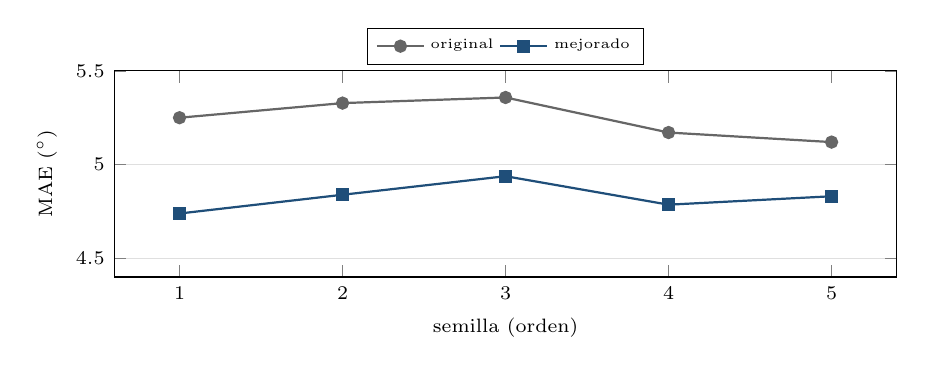
\begin{tikzpicture}
\begin{axis}[width=0.95\textwidth,height=4.2cm,xlabel={semilla (orden)},ylabel={\mae{} (\gr)},xtick={1,2,3,4,5},ymin=4.4,ymax=5.5,
 legend style={font=\tiny,at={(0.5,1.03)},anchor=south,legend columns=2},tick label style={font=\scriptsize},label style={font=\scriptsize},ymajorgrids,grid style={gray!25}]
\addplot[gris,mark=*,thick] coordinates {(1,5.250)(2,5.328)(3,5.358)(4,5.171)(5,5.120)};
\addplot[azul,mark=square*,thick] coordinates {(1,4.739)(2,4.839)(3,4.938)(4,4.786)(5,4.831)};
\legend{original,mejorado}
\end{axis}
\end{tikzpicture}
\end{column}
\end{columns}
\end{frame}

%--------------------------------------------------------------------
\begin{frame}{Modelo A: latente de 32 números y re-ajuste del cierre}
\begin{columns}[T]
\begin{column}{0.4\textwidth}
\begin{itemize}\setlength{\itemsep}{4pt}\small
\item Con latente 16 el mejor peso era $w=0.05$; con 32, $w=0.1$.
\item Con más capacidad, la red puede ``sortear'' el cierre con más detalle; la penalización debe ser más exigente.
\end{itemize}
\small
\begin{tabular}{lcc}
\toprule
 & \mae{} & Salto\\
\midrule
16, $w{=}0.05$ & $4.20\pm0.03$ & $1.33\pm0.15$\\
\rowcolor{verdec}32, $w{=}0.1$ & \bpm{4.11}{0.05} & \bpm{0.87}{0.11}\\
$p$ & \textbf{0.018} & \textbf{0.004}\\
\bottomrule
\end{tabular}

\vspace{4pt}
\begin{alertblock}{Lección}\scriptsize
Los hiperparámetros dependen entre sí. Cambiar el latente sin re-ajustar $w$ habría conducido a una conclusión errónea.
\end{alertblock}
\end{column}
\begin{column}{0.58\textwidth}
\centering
\pgfplotsset{semilla/.style={width=0.5\textwidth,height=4.8cm,xtick={1,2,3,4,5},tick label style={font=\scriptsize},label style={font=\scriptsize},ymajorgrids,grid style={gray!25},legend style={font=\tiny}}}
\begin{tikzpicture}
\begin{axis}[semilla,xlabel={semilla (orden)},ylabel={\mae{} (\gr)},ymin=4.0,ymax=4.3,title={\scriptsize Error},legend pos=north east]
\addplot[azulm,mark=*,thick] coordinates {(1,4.182)(2,4.208)(3,4.234)(4,4.178)(5,4.176)};
\addplot[azul,mark=square*,thick] coordinates {(1,4.038)(2,4.163)(3,4.118)(4,4.147)(5,4.099)};
\legend{16,32}
\end{axis}
\end{tikzpicture}\hspace{-0.2cm}\begin{tikzpicture}
\begin{axis}[semilla,xlabel={semilla (orden)},ylabel={salto (\gr)},ymin=0.6,ymax=1.6,title={\scriptsize Salto de cierre}]
\addplot[azulm,mark=*,thick] coordinates {(1,1.140)(2,1.494)(3,1.198)(4,1.358)(5,1.433)};
\addplot[azul,mark=square*,thick] coordinates {(1,0.968)(2,0.985)(3,0.771)(4,0.759)(5,0.843)};
\end{axis}
\end{tikzpicture}

{\scriptsize El latente 32 gana en las 5 semillas en ambas métricas.}
\end{column}
\end{columns}
\end{frame}

%--------------------------------------------------------------------
\begin{frame}{Ensamble de cinco semillas}
\begin{columns}[T]
\begin{column}{0.48\textwidth}
\begin{block}{Idea}
Entrenar 5 modelos con semillas distintas y \alert{promediar sus salidas}.
\end{block}
\begin{itemize}\setlength{\itemsep}{4pt}\small
\item Cada modelo se equivoca algo distinto por azar; al promediar, el azar se cancela parcialmente, como al promediar varias mediciones.
\item Lo que \emph{no} se cancela es un error sistemático (compartido por todos).
\item Por eso mezclar modelos de objetivos distintos (A y B) da un resultado intermedio, no mejor.
\end{itemize}
\end{column}
\begin{column}{0.48\textwidth}
\small
\begin{tabular}{lccc}
\toprule
 & \textbf{\mae{}} & \textbf{Salto} & \textbf{Corr.}\\
\midrule
A, 1 modelo & 4.11 & 0.87 & --\\
\rowcolor{verdec}A, ensamble & \textbf{3.91} & 0.55 & 0.229\\
B, 1 modelo & 4.83 & 0.57 & 0.337\\
\rowcolor{verdec}B, ensamble & 4.74 & \textbf{0.36} & \textbf{0.349}\\
A + B (10 modelos) & 4.16 & 0.39 & 0.319\\
\bottomrule
\end{tabular}

\vspace{4pt}
{\scriptsize A: entrenado con ciclos limpios. B: con ciclos dañados. Un solo ensamble por fila; su incertidumbre no fue medida. Negrilla: mejor valor de la columna.}
\end{column}
\end{columns}
\end{frame}

%--------------------------------------------------------------------
\begin{frame}{Lo que no funcionó (y qué enseña)}
\scriptsize
\renewcommand{\arraystretch}{1.12}
\begin{tabularx}{\textwidth}{@{}>{\raggedright\arraybackslash}p{3.2cm}>{\raggedright\arraybackslash}X>{\raggedright\arraybackslash}p{4.6cm}@{}}
\toprule
\textbf{Experimento} & \textbf{Resultado} & \textbf{Explicación probable}\\
\midrule
Decodificador bidireccional & \mae{} 4.244 / salto 3.920 frente a 4.219 / 3.912 (misma configuración, sin cierre) & Ya recibe $z$ y fase en cada paso; mirar hacia atrás no agrega información\\
Atención en el codificador & \mae{} $\approx8.5$\gr; pesos casi uniformes ($\approx1/101$) & Con 240 ciclos no se aprende dónde mirar; degenera en promedio\\
Velocidad angular como entrada & \mae{} 4.728 $\to$ 4.822 & La derivada amplifica el ruido de la estimación por video\\
Asimetría izquierda-derecha & \mae{} 4.728 $\to$ 4.771 & La información ya está en los seis canales\\
Consistencia del latente & \mae{} 4.833 vs 4.835 ($p=0.85$) & El denoising ya induce códigos parecidos\\
Intensidad de corrupción & Corrección 0.320 / 0.349 / 0.329 para intensidad 0.5 / 1.0 / 1.5 (\mae{} 4.45 / 4.73 / 5.12) & U invertida: óptimo en 1.0; la receta original estaba calibrada\\
Currículo de corrupción & \mae{} $4.83\to4.79$ ($p=0.26$) & Dentro del ruido entre semillas\\
Ensamble mixto A + B & \mae{} 4.16, corrección 0.319 (intermedio) & Objetivos distintos; ver ``Dos modelos, dos trabajos''\\
\bottomrule
\end{tabularx}
\end{frame}

%--------------------------------------------------------------------
\begin{frame}{Conclusión de los resultados negativos}
\begin{columns}[T]
\begin{column}{0.56\textwidth}
\begin{block}{Lectura de conjunto}
Casi toda adición de componentes aprendibles (atención, más entradas, términos extra) \alert{no aportó}. El cuello de botella parece ya no ser la arquitectura sino el \textbf{tamaño de los datos}: 240 ciclos de 28 personas.
\end{block}
\begin{itemize}\setlength{\itemsep}{3pt}\small
\item Con pocos datos, agregar parámetros agrega más ruido que señal.
\item Las dos mejoras que funcionaron son \emph{restricciones} simples (entregar $z$, cerrar el ciclo), no componentes nuevos.
\end{itemize}
\end{column}
\begin{column}{0.4\textwidth}
\begin{exampleblock}{Implicación}
Los próximos avances más probables provienen de:
\begin{itemize}\setlength{\itemsep}{1pt}\small
\item más datos o aumento de datos realista,
\item restricciones físicas adicionales,
\item mejor selección de hiperparámetros (validación cruzada por sujeto).
\end{itemize}
\end{exampleblock}
\end{column}
\end{columns}
\end{frame}

%--------------------------------------------------------------------
\begin{frame}{Dos modelos, dos trabajos}
\begin{columns}[T]
\begin{column}{0.58\textwidth}
\small
\begin{tabularx}{\textwidth}{@{}>{\bfseries}p{2.2cm}>{\raggedright\arraybackslash}X>{\raggedright\arraybackslash}X@{}}
\toprule
 & \textbf{A} (ciclos limpios) & \textbf{B} (ciclos dañados)\\
\midrule
Entrenamiento & ciclo limpio $\to$ mismo ciclo & ciclo dañado $\to$ ciclo limpio\\
Pregunta & ¿Qué tan fielmente se reconstruye? & ¿Cómo sería la versión típica?\\
Fortaleza & mejor \mae{} de las dos (\textbf{3.91\gr}, ensamble) & mejor corrección de las dos (\textbf{0.349}, ensamble)\\
Riesgo & reproduce también lo anómalo & se aleja algo de la entrada\\
\bottomrule
\end{tabularx}

\vspace{6pt}
\begin{block}{Analogía}
A es una fotocopiadora de alta calidad (copia incluso los defectos). B es un restaurador (devuelve cómo debería verse). Un ensamble mixto es una fotocopiadora que a veces restaura: queda en un punto intermedio (\mae{} 4.16\gr, corrección 0.319).
\end{block}
\end{column}
\begin{column}{0.4\textwidth}
\begin{alertblock}{¿Por qué no PCA (\mae{} 2.78\gr)?}\footnotesize
PCA reproduce muy bien, pero justamente por eso reproduce también lo atípico: su ganancia de tipicidad es la más baja de la comparación (0.127, frente a 0.349 y 0.385 de A y B originales).

\smallskip
Para fidelidad pura, PCA sigue siendo superior; el RNN aún no la alcanza. B supera a PCA en corrección (0.349 frente a 0.207), pero queda por debajo del autoencoder convolucional denoising del cuaderno original (0.412).\par\smallskip\textit{Nota}: la tipicidad alta de A original (0.349) coincide con una intervención grande (8.12\gr) por su error alto; no es corrección deliberada.
\end{alertblock}
\end{column}
\end{columns}
\end{frame}

%--------------------------------------------------------------------
\begin{frame}{Escalera de mejora: error de reconstrucción}
\centering
\small\textbf{\mae{} en el conjunto de control (grados; menor es mejor)}

\vspace{4pt}
\barchart{A original (cuaderno)/5.17/0, A original (reproducido)/4.99/0, A: código por paso y cierre/4.20/1, A: latente 32 y $w{=}0.1$/4.11/1, A: ensamble de 5/3.91/1, B original (cuaderno)/5.35/0, B: código por paso y cierre/4.83/1, B: ensamble de 5/4.74/1, Proceso gaussiano/3.30/0, PCA/2.78/0}{1.9cm}{0.40cm}

\vspace{4pt}
{\scriptsize Gris: referencias. Azul: versiones mejoradas. Barras de un modelo = promedio de 5 semillas; ``ensamble'' = un ensamble de 5.}
\end{frame}

%--------------------------------------------------------------------
\begin{frame}{Escalera de mejora: cierre del ciclo}
\centering
\small\textbf{Salto entre el punto 0\% y el 100\% (grados; menor es mejor)}

\vspace{4pt}
\barchart{A original (cuaderno)/4.94/0, A original (reproducido)/5.07/0, A: código por paso y cierre/1.33/1, A: latente 32 y $w{=}0.1$/0.87/1, A: ensamble de 5/0.55/1, B original (cuaderno)/3.45/0, B: código por paso y cierre/0.57/1, B: ensamble de 5/0.36/1, Proceso gaussiano/0.60/0, PCA/3.41/0}{1.9cm}{0.40cm}

\vspace{4pt}
{\scriptsize El salto de los modelos mejorados cae a 0.4--0.9\gr\ ($-82$ a $-90\%$); B y los ensambles igualan o superan al proceso gaussiano periódico (0.60\gr), y A en un modelo (0.87\gr) queda algo por encima.}
\end{frame}

%--------------------------------------------------------------------
\begin{frame}{Cuánto se mejoró}
\begin{columns}[T]
\begin{column}{0.56\textwidth}
\footnotesize\setlength{\tabcolsep}{3.5pt}
\begin{tabular}{@{}lccc@{}}
\toprule
 & \textbf{Inicial} & \textbf{1 modelo} & \textbf{Ensamble de 5}\\
\midrule
A: \mae{} (\gr) & 5.17 & 4.11 ($-20\%$) & \textbf{3.91} ($-24\%$)\\
A: salto (\gr) & 4.94 & 0.87 ($-82\%$) & \textbf{0.55} ($-89\%$)\\
B: \mae{} (\gr) & 5.35 & 4.83 ($-10\%$) & \textbf{4.74} ($-11\%$)\\
B: salto (\gr) & 3.45 & 0.57 ($-84\%$) & \textbf{0.36} ($-90\%$)\\
B: corrección & 0.280 & 0.337 ($+20\%$) & \textbf{0.349} ($+25\%$)\\
\bottomrule
\end{tabular}

\vspace{4pt}
{\scriptsize 1 modelo: promedio de 5 modelos entrenados por separado (cifra validada). Ensamble: promedio de las predicciones de esos 5 modelos; es mejor, pero proviene de un único ensamble y cuesta cinco modelos. Negrilla: mejor cifra de cada fila.}
\end{column}
\begin{column}{0.41\textwidth}
\begin{alertblock}{Dos comparaciones posibles}\small
Los porcentajes comparan contra las cifras del cuaderno inicial.

Contra la \emph{reproducción} del modelo inicial con el mismo protocolo (4.99 y 5.25 de \mae{}), la mejora en fidelidad es algo menor: $-18\%$ (A) y $-8\%$ (B).

La segunda comparación es la más estricta.
\end{alertblock}
\end{column}
\end{columns}
\end{frame}

%--------------------------------------------------------------------
\begin{frame}{Veredicto: qué modelo es mejor y cuánto mejoró}
\begin{block}{Respuesta directa}
El \textbf{modelo A mejorado es el mejor para reconstruir} y el \textbf{modelo B mejorado es el mejor para corregir}; ninguno gana en todo. Con ensamble de 5, A alcanzó un \mae{} de \textbf{3.91\gr} (original 5.17\gr; $-24\%$) y un salto de cierre de \textbf{0.55\gr} (original 4.94\gr; $-89\%$). Con ensamble de 5, B alcanzó una ganancia de corrección de \textbf{0.349} (original 0.280; $+25\%$), con \mae{} de \textbf{4.74\gr} (original 5.35\gr; $-11\%$) y salto de \textbf{0.36\gr} (original 3.45\gr; $-90\%$). Como modelo individual: A, 4.11\gr\ y 0.87\gr; B, corrección 0.337, 4.83\gr\ y 0.57\gr.
\end{block}
\vspace{2pt}
\begin{columns}[T]
\begin{column}{0.56\textwidth}
\footnotesize\setlength{\tabcolsep}{3pt}
\begin{tabular}{@{}llcc@{}}
\toprule
\textbf{Objetivo} & \textbf{Mejor} & \textbf{Ensamble (1 modelo)} & \textbf{Rival}\\
\midrule
Fidelidad (\mae{}) & \textbf{A} & \textbf{3.91\gr} (4.11\gr) & B: 4.74\gr\\
Cierre (salto) & \textbf{B} & \textbf{0.36\gr} (0.57\gr) & A: 0.55\gr\\
Corrección & \textbf{B} & \textbf{0.349} (0.337) & A: 0.229\\
\bottomrule
\end{tabular}
\end{column}
\begin{column}{0.42\textwidth}
\begin{alertblock}{Salvedades}\scriptsize
PCA sigue mejor en \mae{} (2.78\gr); el autoencoder convolucional denoising sigue mejor corrigiendo (0.412). A no mejoró su corrección (0.208 $\to$ 0.189; $p=0.077$) y su tipicidad bajó algo (0.345 $\to$ 0.326). Un codificador lineal con el mismo decodificador alcanza 3.26\gr\ de \mae{} en ensamble (control).
\end{alertblock}
\end{column}
\end{columns}
\end{frame}

%--------------------------------------------------------------------
\begin{frame}{Entonces, ¿por qué no PCA ni el convolucional denoising?}
\begin{columns}[T]
\begin{column}{0.5\textwidth}
\footnotesize\setlength{\tabcolsep}{3pt}
\begin{tabular}{@{}lccc@{}}
\toprule
 & \textbf{\mae{} (\gr)} & \textbf{Salto (\gr)} & \textbf{Corr.}\\
\midrule
PCA & \textbf{2.78} & 3.41 & 0.207\\
Proceso gaussiano periódico & 3.30 & 0.60 & 0.215\\
Conv. denoising & 4.07 & 1.88 & \textbf{0.412}\\
\rowcolor{verdec}A mejorado (ensamble) & 3.91 & 0.55 & 0.229\\
\rowcolor{verdec}B mejorado (ensamble) & 4.74 & \textbf{0.36} & 0.349\\
\bottomrule
\end{tabular}

\vspace{3pt}
{\scriptsize Negrilla: mejor valor de la columna. RNN: un único ensamble tras las mejoras; resto: cuaderno original, una corrida.}

\vspace{4pt}
\begin{alertblock}{Conclusión}\small
Con las cifras actuales \textbf{no hay una razón basada en métricas} para preferir la RNN: PCA gana en fidelidad y el convolucional denoising en corrección. La RNN solo queda al frente en cierre de ciclo, y por poco.
\end{alertblock}
\end{column}
\begin{column}{0.48\textwidth}
\begin{block}{La comparación favorece a la RNN}\scriptsize
Sus hiperparámetros fueron afinados sobre el conjunto de control; los de PCA y del convolucional no, y sus cifras son de una sola corrida. Aun así, la RNN no los supera.
\end{block}
\begin{block}{Razones posibles para mantener la RNN}\scriptsize
Decisión de diseño del proyecto, o necesidades de la aplicación (dinámica en el tiempo, ciclos de distinta longitud). Ninguna fue medida; debe ser confirmada.
\end{block}
\begin{exampleblock}{Propuesta}\scriptsize
\begin{enumerate}\setlength{\itemsep}{1pt}
\item Definir si se mejora la RNN por diseño o se busca el mejor modelo.
\item Aplicar cierre de ciclo (y código por paso) al convolucional denoising.
\item Reevaluar PCA y el convolucional con 5 semillas y el mismo protocolo.
\end{enumerate}
\end{exampleblock}
\end{column}
\end{columns}
\end{frame}

%--------------------------------------------------------------------
\begin{frame}{Experimento adicional: modelo fundacional como codificador}
\centering
\resizebox{\textwidth}{!}{%
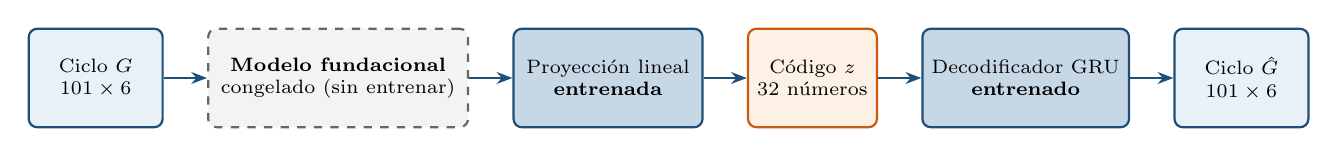
\begin{tikzpicture}[node distance=0.55cm,
 caja/.style={draw=azul,fill=azulc,rounded corners=3pt,minimum height=1.25cm,align=center,font=\scriptsize,thick},
 flecha/.style={-{Stealth[length=2mm]},thick,azul}]
\node[caja,minimum width=1.7cm] (in) {Ciclo $G$\\ $101\times6$};
\node[draw=gris,dashed,fill=grisc,rounded corners=3pt,thick,minimum height=1.25cm,right=of in,minimum width=3.3cm,align=center,font=\scriptsize] (tf) {\textbf{Modelo fundacional}\\ congelado (sin entrenar)};
\node[caja,right=of tf,minimum width=2.4cm,fill=azulm!35] (pr) {Proyección lineal\\ \textbf{entrenada}};
\node[draw=naranja,fill=naranjac,thick,rounded corners=3pt,right=of pr,minimum width=1.3cm,minimum height=1.25cm,align=center,font=\scriptsize] (z) {Código $z$\\ 32 números};
\node[caja,right=of z,minimum width=2.4cm,fill=azulm!35] (dec) {Decodificador GRU\\ \textbf{entrenado}};
\node[caja,right=of dec,minimum width=1.7cm] (out) {Ciclo $\hat G$\\ $101\times6$};
\draw[flecha] (in)--(tf); \draw[flecha] (tf)--(pr); \draw[flecha] (pr)--(z); \draw[flecha] (z)--(dec); \draw[flecha] (dec)--(out);
\end{tikzpicture}}

\vspace{6pt}
\begin{columns}[T]
\begin{column}{0.5\textwidth}
\begin{block}{Idea y diseño}\scriptsize
Se evalúa si las representaciones de un modelo de series de tiempo preentrenado (TimesFM 2.5, 200 millones de parámetros) sirven como código del ciclo.
\begin{itemize}\setlength{\itemsep}{1pt}
\item Cada canal se remuestrea a 128 puntos (4 parches). Del estado interno de un bloque se promedian los parches y se toma el último; se añaden la media y la desviación de la serie, que el modelo descarta al normalizar.
\item Se entrenan solo la proyección lineal y el decodificador (el de la mejora 1, con cierre).
\item Mismos datos, partición, pérdida, métricas y 5 semillas que el modelo mejorado. Tipo A: latente 32, $w=0.1$. Tipo B: latente 16, $w=0.05$.
\item La configuración (bloque, agrupación, decaimiento de pesos) fue elegida solo con validación, con una semilla.
\end{itemize}
\end{block}
\end{column}
\begin{column}{0.48\textwidth}
\begin{alertblock}{Dos controles}\scriptsize
\begin{itemize}\setlength{\itemsep}{1pt}
\item \textbf{Pesos aleatorios:} misma arquitectura sin preentrenar (normas internas con escala uno). Separa el aporte del preentrenamiento del de la arquitectura.
\item \textbf{Serie cruda:} la serie estandarizada entra directamente a la proyección lineal. Indica qué se logra sin ningún modelo preentrenado.
\end{itemize}
\end{alertblock}
\begin{exampleblock}{Prueba de sanidad de los pesos}\scriptsize
Pronóstico de una onda seno: error de \textbf{0.036} con pesos preentrenados y de 1.877 con pesos aleatorios. Los pesos se cargaron correctamente.
\end{exampleblock}
\end{column}
\end{columns}
\end{frame}

%--------------------------------------------------------------------
\begin{frame}{Resultado: el modelo fundacional congelado no mejora}
\begin{columns}[T]
\begin{column}{0.56\textwidth}
\footnotesize\setlength{\tabcolsep}{2.6pt}
\textbf{Tipo A (autoencoder limpio)}

\begin{tabular}{@{}lcccc@{}}
\toprule
 & \textbf{\mae{} (\gr)} & \textbf{Salto (\gr)} & \textbf{Correc.} & \textbf{Tipic.}\\
\midrule
Preentrenado & 7.19 (6.76) & 2.55 & $-0.149$ & 0.101\\
Pesos aleatorios & 7.23 (6.66) & 2.74 & $-0.017$ & 0.087\\
Serie cruda & \textbf{3.69} (3.26) & 1.40 & 0.011 & 0.181\\
\rowcolor{verdec}GRU mejorado & 4.11 (3.91) & \textbf{0.87} & \textbf{0.189} & \textbf{0.326}\\
\bottomrule
\end{tabular}

\vspace{5pt}
\textbf{Tipo B (con eliminación de ruido)}

\begin{tabular}{@{}lcccc@{}}
\toprule
 & \textbf{\mae{} (\gr)} & \textbf{Salto (\gr)} & \textbf{Correc.} & \textbf{Tipic.}\\
\midrule
Preentrenado & 10.12 (9.76) & 6.80 & $-0.117$ & $-0.049$\\
Serie cruda & \textbf{4.46} (4.33) & 1.28 & \textbf{0.380} & 0.390\\
\rowcolor{verdec}GRU mejorado & 4.83 (4.74) & \textbf{0.57} & 0.337 & \textbf{0.414}\\
\bottomrule
\end{tabular}

\vspace{3pt}
{\scriptsize Promedio de 5 semillas (ensamble de las 5 entre paréntesis, solo \mae{}). Salto: cierre del ciclo. Negrilla: mejor valor de la columna en cada tabla.}
\end{column}
\begin{column}{0.42\textwidth}
\begin{alertblock}{Lectura}\scriptsize
\begin{itemize}\setlength{\itemsep}{2pt}
\item El preentrenamiento \textbf{no aporta en fidelidad}: \mae{} de 7.19\gr\ con pesos preentrenados y 7.23\gr\ con aleatorios ($p=0.83$). El salto no difiere ($p=0.19$) y la corrección es peor con pesos preentrenados ($p=0.004$).
\item Es peor que el GRU mejorado en fidelidad, cierre, corrección y tipicidad ($p\le0.003$, 5 semillas, sin corrección por multiplicidad).
\item Tipo B: entrenamiento detenido pronto (20 a 42 épocas) y corrección negativa.
\end{itemize}
\end{alertblock}
\begin{block}{Alcance de la conclusión}\scriptsize
Vale para este diseño (un modelo, representaciones congeladas agrupadas, proyección lineal, 240 ciclos de entrenamiento y 15\,372 características). No se probaron otros modelos, conservar los cuatro parches ni afinar el codificador.
\end{block}
\end{column}
\end{columns}
\end{frame}

%--------------------------------------------------------------------
\begin{frame}{Hallazgo de los controles: un codificador lineal basta}
\begin{columns}[T]
\begin{column}{0.54\textwidth}
\footnotesize\setlength{\tabcolsep}{3pt}
\begin{tabular}{@{}llccc@{}}
\toprule
 & & \textbf{Lineal} & \textbf{GRU} & \textbf{$p$}\\
\midrule
\multirow{4}{*}{A} & \mae{} (\gr) & \textbf{3.69} & 4.11 & 0.002\\
 & Salto (\gr) & 1.40 & \textbf{0.87} & 0.001\\
 & Corrección & 0.011 & \textbf{0.189} & $<0.001$\\
 & Tipicidad & 0.181 & \textbf{0.326} & $<0.001$\\
\midrule
\multirow{4}{*}{B} & \mae{} (\gr) & \textbf{4.46} & 4.83 & $<0.001$\\
 & Salto (\gr) & 1.28 & \textbf{0.57} & $<0.001$\\
 & Corrección & \textbf{0.380} & 0.337 & $<0.001$\\
 & Tipicidad & 0.390 & \textbf{0.414} & 0.007\\
\bottomrule
\end{tabular}

\vspace{4pt}
{\scriptsize Lineal: proyección lineal de la serie cruda al código y el mismo decodificador GRU con cierre. GRU: codificador recurrente (modelo mejorado). Promedio de 5 semillas; $p$: prueba t pareada. Negrilla: mejor valor de cada fila.}
\end{column}
\begin{column}{0.44\textwidth}
\begin{block}{Qué indica}\scriptsize
Sustituir el codificador recurrente por una proyección lineal \emph{reduce el error de reconstrucción} en A y B y \emph{mejora la corrección} en B. Entonces, el codificador GRU no parece ser lo que limita el rendimiento; es consistente con que PCA, también lineal, tenga el menor \mae{}.
\end{block}
\begin{alertblock}{Salvedades}\scriptsize
\begin{itemize}\setlength{\itemsep}{1pt}
\item Surgió de un control, no de una hipótesis previa.
\item El lineal pierde en cierre, pendiente de la costura y (en A) en corrección y tipicidad.
\item Los hiperparámetros del GRU fueron afinados sobre el conjunto de control; los del lineal no. La comparación favorece al GRU y aun así pierde en \mae{}.
\end{itemize}
\end{alertblock}
\end{column}
\end{columns}
\end{frame}

%--------------------------------------------------------------------
\begin{frame}{Limitaciones y salvedades}
\begin{columns}[T]
\begin{column}{0.5\textwidth}
\begin{enumerate}\setlength{\itemsep}{3pt}\footnotesize
\item Los hiperparámetros fueron elegidos observando el conjunto de prueba de control; las cifras finales son algo \alert{optimistas}.
\item Los latentes 32/48/64 en el modelo denoising \alert{no se distinguen} (modelos individuales, 16 frente a 32, 5 semillas: \mae{} $p=0.52$; corrección $p=0.18$).
\item Cada ensamble proviene de un único conjunto de 5 modelos.
\end{enumerate}
\end{column}
\begin{column}{0.48\textwidth}
\begin{enumerate}\setlength{\itemsep}{3pt}\footnotesize\setcounter{enumi}{3}
\item La evaluación de corrección usa una sola realización del daño aleatorio (con otra, la corrección de B mejorado pasó de 0.337 a 0.32).
\item Datos reconstruidos de los archivos entregados; las cifras reproducidas difieren algo del cuaderno inicial (4.99 vs 5.17; 5.25 vs 5.35).
\item Otras lecturas de $t$ y $t-1$: validadas solo en A (dos en B); por confirmar.
\item El autoencoder convolucional no se reevaluó con 5 semillas.
\item El experimento con modelo fundacional cubre un solo diseño y un solo modelo; la configuración se eligió con una semilla.
\end{enumerate}
\end{column}
\end{columns}
\vspace{-4pt}
\begin{exampleblock}{Cómo se mitigó}\footnotesize
Partición por sujeto, cinco semillas con prueba pareada para toda afirmación, y reporte explícito de los resultados negativos.
\end{exampleblock}
\end{frame}

%--------------------------------------------------------------------
\begin{frame}{Conclusiones}
\begin{enumerate}\setlength{\itemsep}{4pt}
\item El autoencoder recurrente presentaba \alert{dos defectos concretos}: olvido del código y falta de cierre del ciclo.
\item Entregar $z$ en cada paso y penalizar el salto de cierre redujeron el error ($-20\%$) y el salto ($-82\%$) del modelo A (un modelo), con \alert{menor variabilidad} entre semillas.
\item La misma receta mejoró el modelo B (un modelo): cierre ($-84\%$) y corrección ($+20\%$); en ensamble, corrección $+25\%$.
\item A (fidelidad, \mae{} 3.91\gr\ en ensamble) y B (corrección, 0.349 en ensamble) cumplen funciones distintas y no deben mezclarse.
\item La mayoría de las ideas adicionales no aportó; el límite actual parece ser la \alert{cantidad de datos}.
\item La fidelidad de PCA (2.78\gr) aún no fue alcanzada por el RNN, aunque PCA no corrige hacia lo típico.
\item Un modelo fundacional congelado (TimesFM) \alert{no mejoró}: su \mae{} fue igual al de pesos aleatorios y peor que el del GRU. Un codificador lineal sobre la serie cruda superó al codificador GRU en \mae{}.
\end{enumerate}
\end{frame}

%--------------------------------------------------------------------
\begin{frame}{Preguntas para discusión y próximos pasos}
\begin{columns}[T]
\begin{column}{0.5\textwidth}
\begin{block}{Preguntas abiertas}
\begin{itemize}\setlength{\itemsep}{3pt}\small
\item De las lecturas probadas de $t$ y $t-1$, ¿cuál se acerca más a lo previsto? ¿Interesa más la forma de la curva o el error?
\item ¿Qué error de reconstrucción o de corrección resulta suficiente para la aplicación?
\item ¿Se prioriza fidelidad (A) o corrección (B) como modelo de referencia?
\item ¿Se mejora la RNN por diseño o se busca el mejor modelo (PCA gana en fidelidad; el convolucional denoising, en corrección)? Dado que un codificador lineal basta, ¿se mantiene el codificador recurrente?
\end{itemize}
\end{block}
\end{column}
\begin{column}{0.48\textwidth}
\begin{exampleblock}{Próximos pasos propuestos}
\begin{enumerate}\setlength{\itemsep}{3pt}\small
\item Aplicar las mejoras al convolucional denoising y reevaluarlo, con PCA, con 5 semillas.
\item Validación cruzada por sujeto para elegir hiperparámetros.
\item Repetir ensambles para medir su incertidumbre y decidir entre latentes 32/48/64.
\item Evaluar los modelos finales en casos externos (evaluación III).
\item Explorar más datos o aumento de datos realista.
\item Probar variantes del modelo fundacional (sin promediar los parches, otros modelos) y medir el codificador lineal con ajuste propio.
\end{enumerate}
\end{exampleblock}
\end{column}
\end{columns}
\end{frame}

%--------------------------------------------------------------------
\appendix
\begin{frame}{Anexo: resultados por semilla (modelo denoising)}
\centering\small
\begin{tabular}{rcccccc}
\toprule
 & \multicolumn{2}{c}{\mae{} (\gr)} & \multicolumn{2}{c}{Salto (\gr)} & \multicolumn{2}{c}{Corrección}\\
\cmidrule(lr){2-3}\cmidrule(lr){4-5}\cmidrule(lr){6-7}
Semilla & inicial & mejorado & inicial & mejorado & inicial & mejorado\\
\midrule
42 & 5.250 & 4.739 & 3.194 & 0.590 & 0.298 & 0.348\\
1 & 5.328 & 4.839 & 3.418 & 0.598 & 0.281 & 0.332\\
7 & 5.358 & 4.938 & 3.040 & 0.525 & 0.283 & 0.333\\
123 & 5.171 & 4.786 & 2.998 & 0.512 & 0.304 & 0.333\\
2024 & 5.120 & 4.831 & 2.569 & 0.611 & 0.313 & 0.339\\
\midrule
Media $\pm$ d.e. & $5.25\pm0.10$ & \bpm{4.83}{0.07} & $3.04\pm0.31$ & \bpm{0.57}{0.05} & $0.296\pm0.014$ & \bpm{0.337}{0.007}\\
\bottomrule
\end{tabular}
\end{frame}

\begin{frame}{Anexo: ensambles y peso de cierre (denoising)}
\begin{columns}[T]
\begin{column}{0.5\textwidth}
\centering\small\textbf{Ensambles de 5 modelos}

\begin{tabular}{lccc}
\toprule
Configuración & \mae{} & Salto & Corr.\\
\midrule
16, $w=0.05$ & 4.743 & 0.361 & 0.349\\
16, $w=0.07$ & 4.746 & 0.290 & 0.349\\
32, $w=0.1$ & 4.682 & 0.286 & 0.357\\
48, $w=0.1$ & 4.670 & \textbf{0.248} & 0.359\\
64, $w=0.1$ & \textbf{4.554} & 0.304 & \textbf{0.369}\\
\bottomrule
\end{tabular}

{\scriptsize Un ensamble por fila; no se midió cuánto varía un ensamble de otro, así que no se sabe si las diferencias son reales. Negrilla: mejor valor de la columna.}
\end{column}
\begin{column}{0.48\textwidth}
\centering\small\textbf{Peso de cierre (latente 16, una semilla)}

\begin{tabular}{lccc}
\toprule
$w$ & \mae{} & Salto & Corr.\\
\midrule
0.02 & 4.731 & 1.002 & 0.347\\
0.03 & 4.729 & 0.693 & \textbf{0.349}\\
0.05 & 4.741 & 0.585 & 0.348\\
0.07 & \textbf{4.728} & 0.460 & \textbf{0.349}\\
0.10 & 4.753 & 0.624 & 0.346\\
0.15 & 4.787 & \textbf{0.324} & 0.343\\
\bottomrule
\end{tabular}

{\scriptsize Con 5 semillas, $w=0.07$ reduce el salto ($0.57\to0.47$, $p=0.022$) sin cambiar \mae{}.}
\end{column}
\end{columns}
\end{frame}

\end{document}
